%% The following is a directive for TeXShop to indicate the main file
%%!TEX root = main.tex

% ===========================================================================================
\chapter{\textbf{Experimental Setup}}
\label{sec4:ExperimentalDetail}

This chapter first describes the details of the two test-beds on which \ac{CORGIDS} was tested then discusses the experimental procedures that were chosen. 

\section{Test-beds}
To demonstrate that \ac{CORGIDS} is generic, two \ac{CPS} test-beds were chosen on which the experiments were carried out. These test-beds contain correlated properties and a predefined framework according to which the properties change their values. 

\begin{enumerate}
\item \acf{UAV}: 
An \ac{UAV}, commonly known as a drone, is a type of aircraft different from others mainly because it does not have a pilot aboard. \ac{UAV} periodically send the flight data to the \ac{GCS} to keep it updated about its whereabouts.
 
An \ac{UAV} mainly consists of sensors, control logic and actuators forming a closed loop. The sensors sense the current state of the \ac{UAV} and its environment and pass it on to the controller, which makes the decision about the next step to be taken. The decision taken is then sent to the actuator - this loop runs infinitely while the \ac{UAV} is in operation. ArduPilot's \acf{SITL} ~\cite{ArdupilotSITL} was used for the experiments. ArduPilot is an open-source autopilot software and is vastly deployed on various vehicle systems. \ac{SITL} was chosen as the test-bed on a local machine due to lack of a real \ac{UAV}.  


\begin{figure}%
    \centering
    \subfloat[Real drone]{{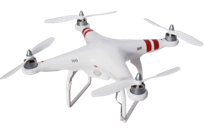
\includegraphics[width=5cm]{Graphics/drone.png} }}%
    \qquad
    \subfloat[ArduPilot's SITL]{{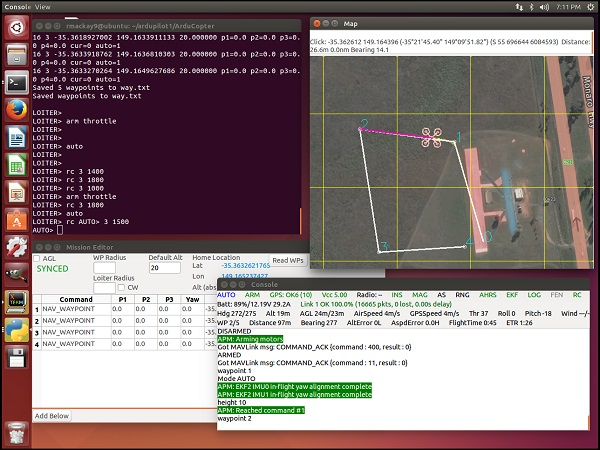
\includegraphics[width=7cm]{Graphics/sitl.jpg} }}%
    \caption{Drones}%
    \label{fig:drone}%
\end{figure}


\item \acf{SAP}: \ac{SAP} is a medical device used by the diabetic patients to automatically analyze the insulin dosage to be injected based on the blood glucose level. It helps in reducing human error and analyzes the current blood glucose levels regularly at fixed intervals of time. A \ac{SAP} consists mainly of i) a blood glucose monitor, which reads the blood glucose levels of the patients at regular interval of time, ii) a controller, which based on the blood glucose values decides the insulin that needs to be injected, iii) an insulin pump, which based on the value generated by the controller, injects a specific amount of insulin into the patient. \acf{OpenAPS}, an open source \ac{SAP} was used to evaluate \ac{CORGIDS}. \ac{OpenAPS} implements the controller part of the \ac{SAP}, and has been used in prior studies~\cite{aliabadi2017artinali}. As there was no real patient, simulated values from blood glucose monitor and the insulin pump we used for our experiments. The values of blood glucose were taken from the test cases provided by \ac{OpenAPS}, instead from the blood glucose monitor. These values were then served as input to the \ac{OpenAPS} to get the amount of insulin required by the patient. The OpenAPS controller was installed on a Raspberry Pi 3 microprocessor to evaluate the memory and performance overhead of \ac{CORGIDS}.

\begin{figure}[ht]
    \centering
    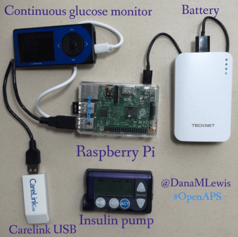
\includegraphics[scale=0.75,keepaspectratio = true]{Graphics/openaps.png}
    \caption{Components of an OpenAPS platform}
    \label{fig:OpenAPS}
\end{figure}
\end{enumerate}

\section{Experimental Procedure}
To evaluate \ac{CORGIDS} efficacy, the process of attack detection was partitioned  into two phases, namely training phase and testing phase. The system traces obtained from \ac{SUT} were randomly divided into training and testing batches. The training phase is the one in which the intrusion detector is trained from the non-faulty system traces that are randomly assigned. Sensitivity analysis is also performed to analyze the value of the parameters which have the most impact on the performance of the intrusion detector. For instance, for the \ac{UAV} testbed, routes which the \ac{UAV} used as the flight plan were randomly generated. Therefore, after having the \ac{UAV} simulator fly on all the randomly generated routes, the non-faulty system traces were obtained. These logs were then randomly distributed for training and testing phases. In the testing phase, the intrusion detector which was built in training phase, was used to find out if an intrusion was correctly detected. The results were then used to gauge the performance of \ac{CORGIDS} based on the evaluation criteria. In order to reduce variability, five-fold cross validation was run for each of the attacks described above.

\endinput
=====================================================================
% EOF